\chapter{Automatic Door Control}

We often come across automatically controlled doors when we enter shopping malls, banks or other such buildings. In this project, we will be developing a similar model on a smaller scale using IR sensor and servo motor.

\subsection*{Components}
\begin{table}[H]
    \centering
    \begin{tabular}{|c|l|c|}\hline
     \textbf{\#} & \textbf{Components} &  \textbf{Amount}\\\hline
     1 & Servo motor &  1\\\hline
     2 & IR transmitter  & 1\\\hline
     3 & IR receiver  &  1\\\hline
     4 & 10 k$\Omega$ resistor  &  1\\\hline
     5 & 470 $\Omega$ resistor   &  1\\\hline
     6 & Arduino UNO & 1 \\\hline
     7 & Connecting wires & - \\\hline
    \end{tabular}
\end{table}

\subsection*{Connections}

\begin{enumerate}[leftmargin=*]
    \item Connect the 470 $\Omega$ resistor with the anode of the IR transmitter and connect its other end with the 5V pin of Arduino. Connect the cathode of the IR transmitter with GND of Arduino.
    \item Connect the cathode of IR receiver with GND of Arduino through a 10 k$\Omega$ resistor. Connect the anode of IR receiver with the 5V pin of Arduino.
    \item Connect the cathode of the IR receiver with A0 pin of Arduino. 
    \item Connect 5V and GND terminals of the servo motor with 3.3 and GND pins of Arduino respectively. 
    \item Connect the PWM wire of the servo motor with pin 9 of Arduino.
  
\end{enumerate}

	\begin{figure}[H]
	\centering 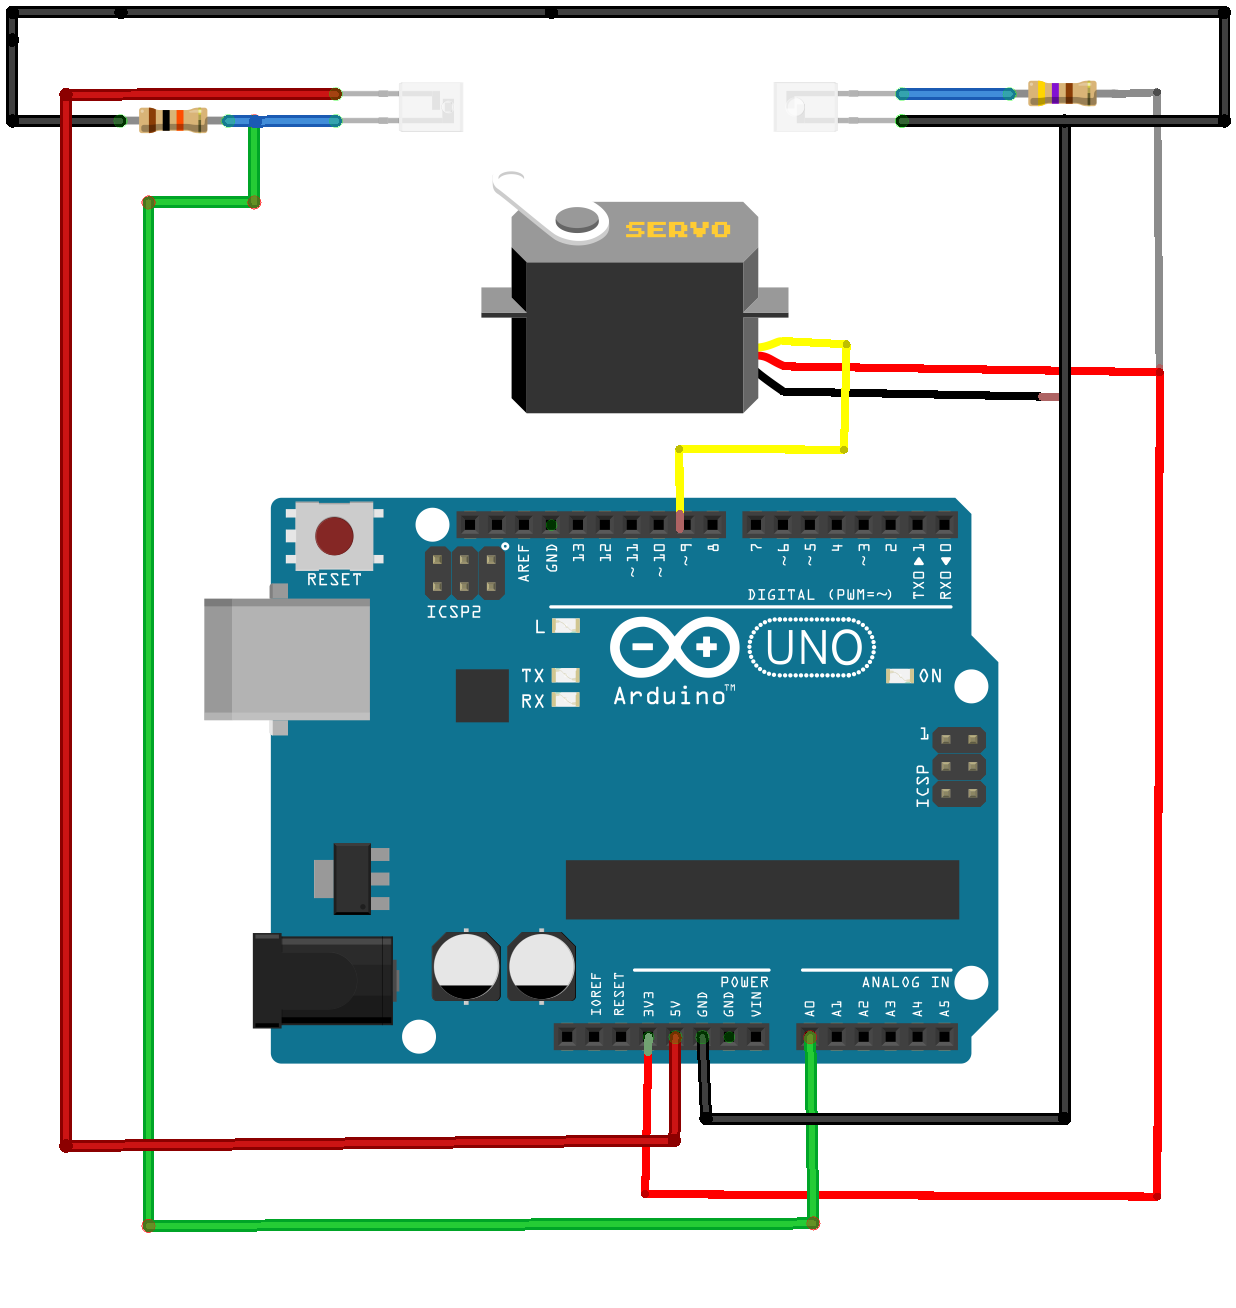
\includegraphics[width=0.4\linewidth]{Figures/recreational_exp/IR serco door_bb.png}
	\caption{Circuit diagram of door controlled using IR}
	\end{figure}
	
\subsection*{Procedure}
\begin{enumerate}[leftmargin=*]
     \item Copy lst. \ref{list:door-with-ir} to a new Arduino sketchbook. Upload the code to your Arduino board.
    \item Interrupt path between IR Receiver and IR Transmitter and observe rotation in the shaft of the servo motor. 
    
\end{enumerate}

\begin{lstlisting}[language=Arduino, numbers=none, caption={Code for door with IR}, captionpos=b, label={list:door-with-ir}]
#include <Servo.h>

// Create servo object 
Servo myservo;  

int servopin = 9; // attaches the servo on pin 9 
int IR= A0; 
int input; // variable to read the value of IR sensor
int threshhold = 1000;

void setup() {
  myservo.attach(servopin);  
}

void loop() {

  input = analogRead(IR);

    if (input > threshhold)
    {
        myservo.write(90);  // Door opens    
    }

    else 
    {
        myservo.write(0);  // Door close
    } 
}
\end{lstlisting}

\begin{figure}[H]
\centering
\begin{subfigure}[b]{0.45\textwidth}
    \centering
    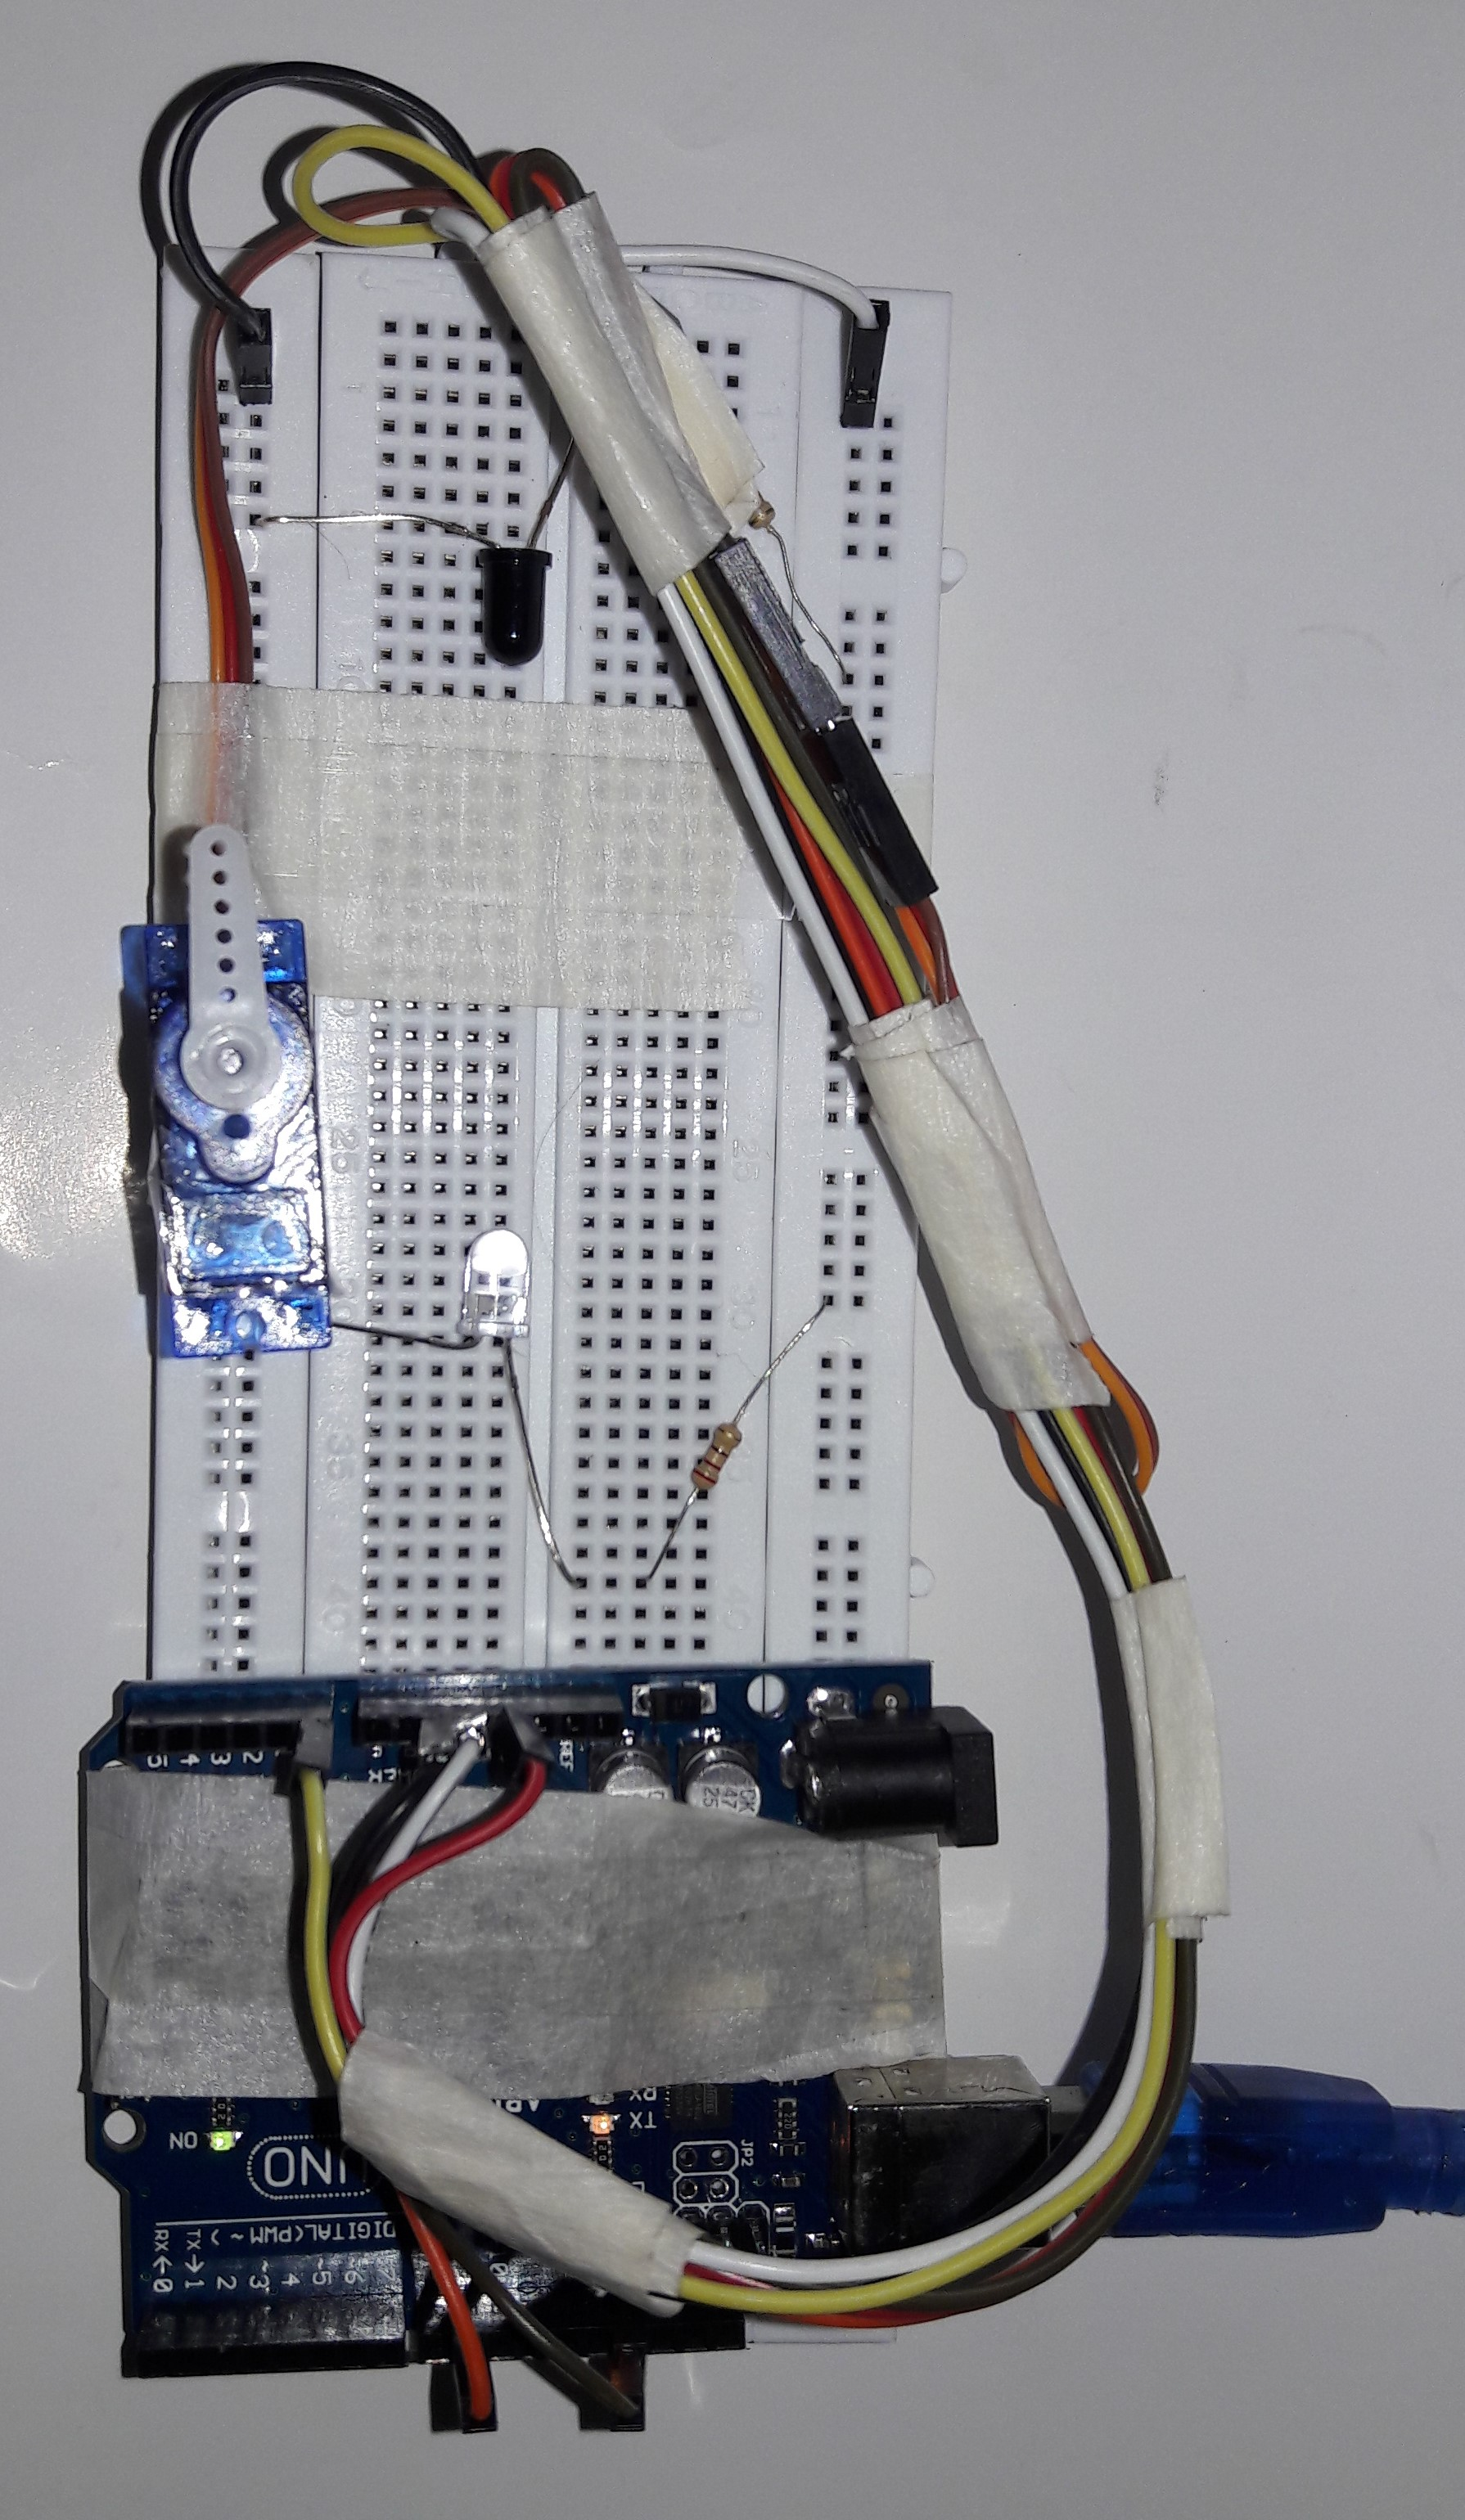
\includegraphics[angle=90, width=\linewidth, height = 0.2\textheight]{Figures/recreational_exp/experiment_pics/IR_servo_door.jpg}
    \end{subfigure}
    \begin{subfigure}[b]{0.45\textwidth}
    \centering
    \raisebox{8mm}[0pt][0pt]
    {
        \parbox[t]{\textwidth}{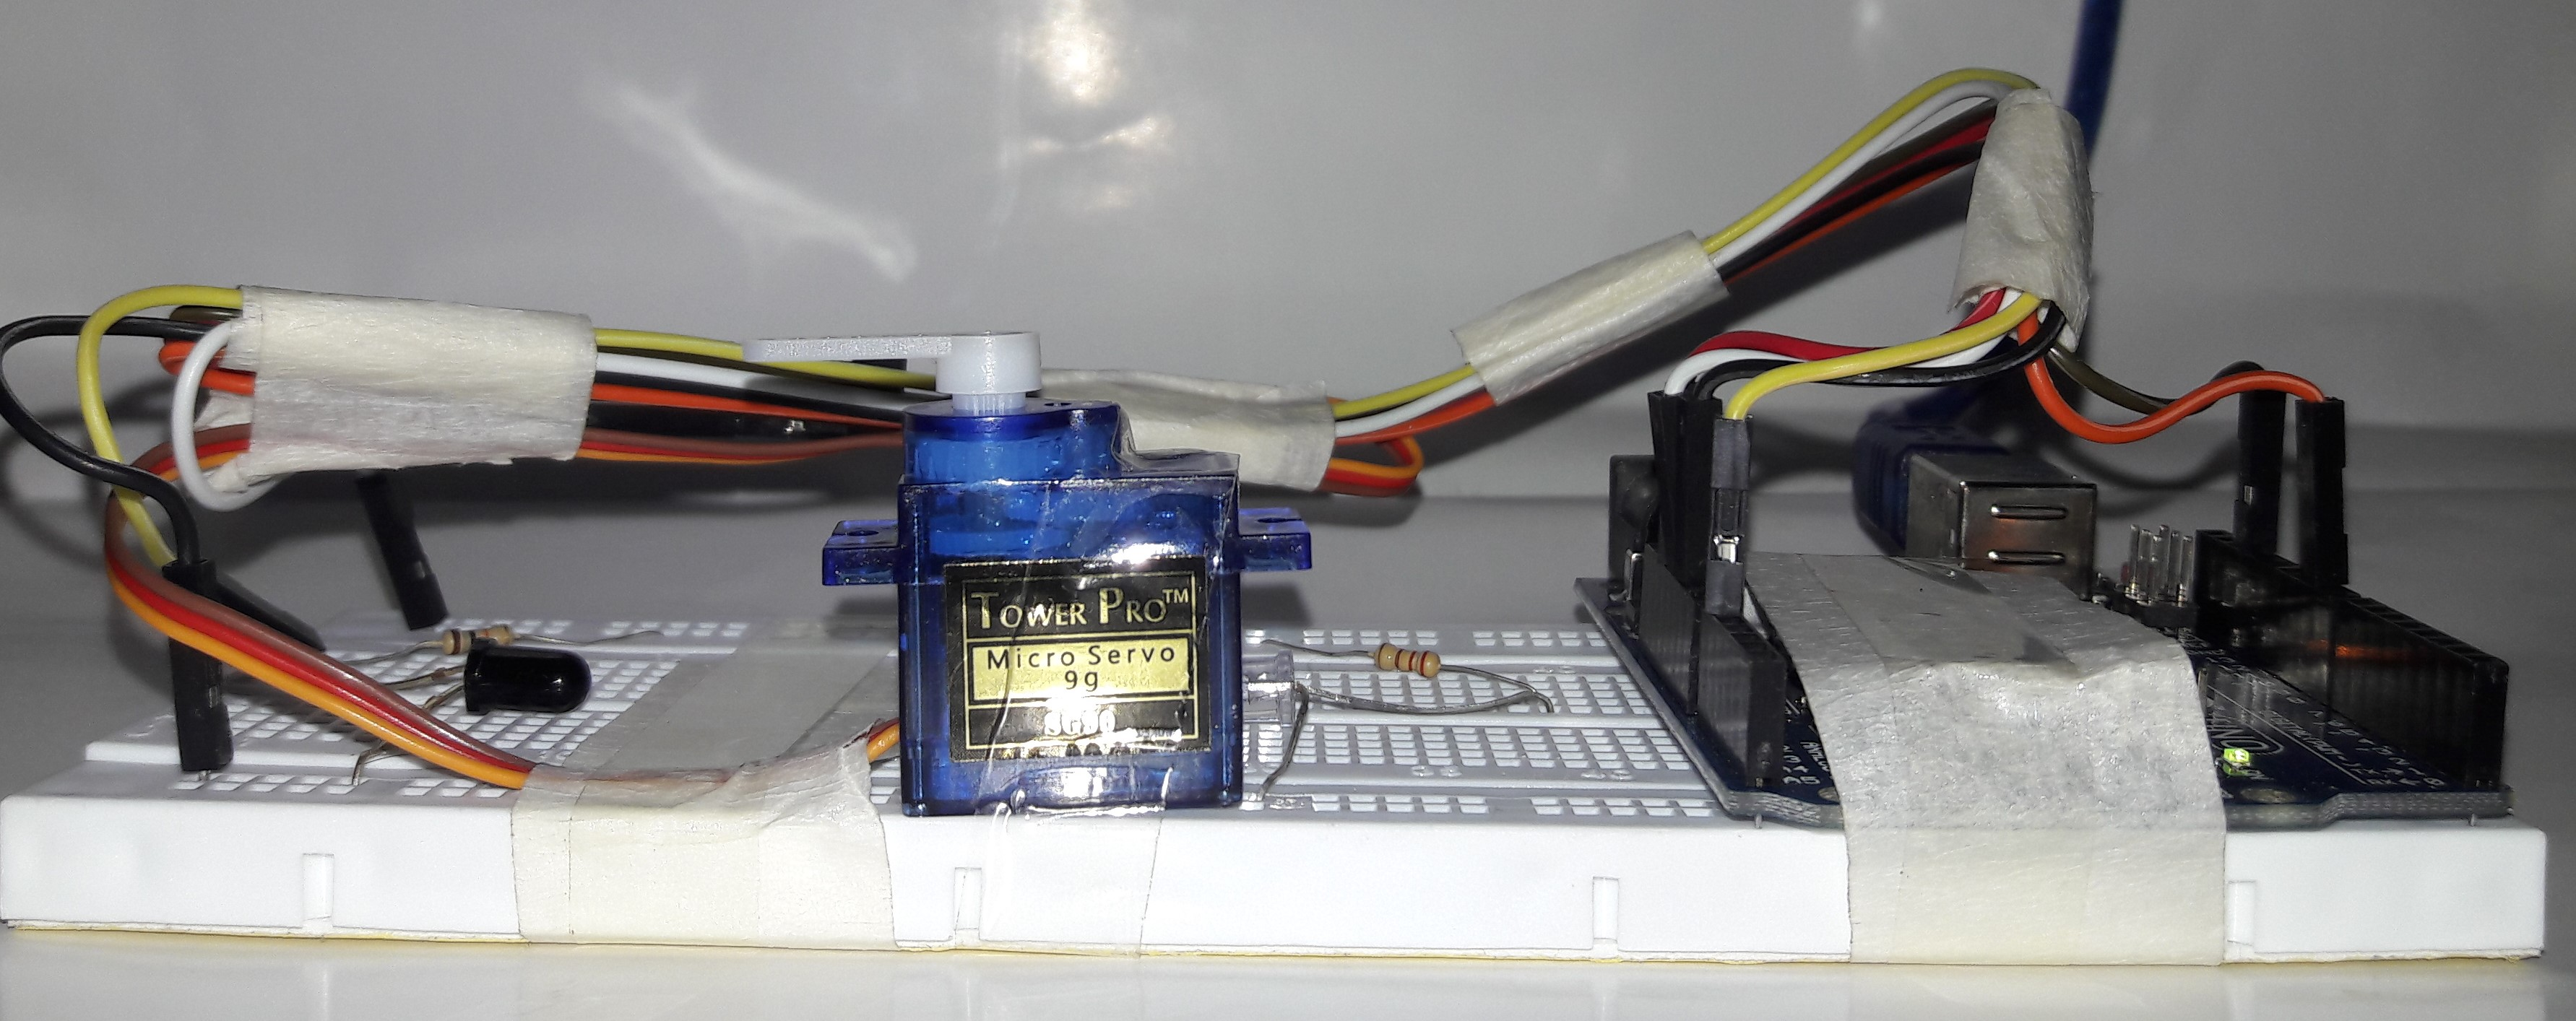
\includegraphics[width=\linewidth]{recreational_exp/experiment_pics/IR_servo_door1.jpg}}
    }
\end{subfigure}
\caption{Hardware of the project}
\end{figure}